% INTRODUÇÃO-------------------------------------------------------------------

\chapter{INTRODUÇÃO}
\label{chap:introducao}

  A luz exerce um papel essencial no nosso cotidiano e está presente das mais diversas formas: iluminação, medicina, pesquisas científicas, geração de energia, telecomunicações, educação, arte, cultura e etc. A Assembleia Geral das Nações Unidas proclamou o ano de 2015 como o Ano Internacional da Luz e das Tecnologias Baseadas na Luz \cite{resolucao-onu}, a fim de reconhecer tal importância para a vida dos cidadãos e para o desenvolvimento futuro da sociedade mundial. No ano da celebração, a UNESCO promoveu uma série de eventos por vários países \citeonline{eventos-unesco}, com o intuito de destacar que o aumento da consciência mundial e o fortalecimento do ensino da ciência e das tecnologias da luz são essenciais para abordar os desafios futuros e atuais, tais como o desenvolvimento sustentável, a energia e as comunicações, assim como para melhorar a qualidade de vida dos países menos desenvolvidos e dos em desenvolvimento.
  
  Baseada em tal iniciativa, a exposição Luz, Ciência e Emoção, idealizada pela arquiteta Dra. Maristela Mitsuko Ono e pelo engenheiro Dr. James Alexandre Baraniuk, traz experimentos envolvendo os conceitos de luz trabalhados nos ensinos pré-escolar e fundamental, cada um com seu grau de impressão aos sentidos. A (\autoref{fig:expo}) apresenta uma parte da mostra que ocorreu entre março e junho de 2017, no Museu de Arte Municipal, em Curitiba.
  
  \begin{figure}[H]%[!htb]
    \centering
    \caption{Parte da exposição ``Luz, Ciência e Emoção'', no MuMa}
    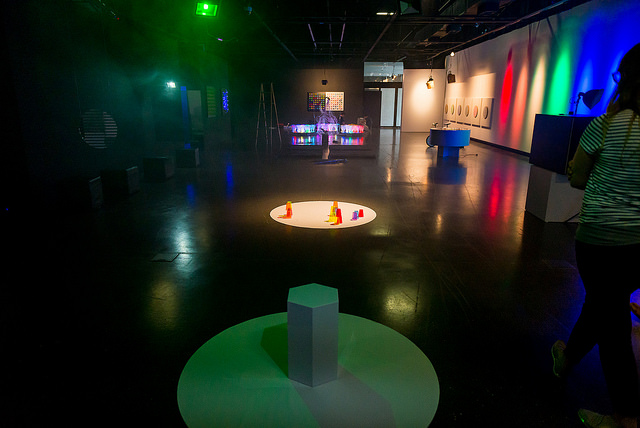
\includegraphics[width=0.95\textwidth]{./dados/figuras/expo}
    \fonte{(UFPR, 2017)}
    \label{fig:expo}
\end{figure}
  
  Dentre outros projetos que participou durante o Programa de Iniciação Científica \footnote{Projeto de Pesquisa: Luz, Ciência e Emoção: Exposição Interativa para Crianças (PIBIC Voluntária: 2016019080)}, o autor trabalhou na seção Matriz da Mesa de Bolinhas (\autoref{fig:mesa-sup}), projeto este que ocupará uma posição de destaque dentro da área artística da mostra. Trata-se de uma matriz de \emph{LEDs} interativa, composta por mais de 100 bolinhas de \emph{ping-pong}, cada uma sobre um correspondente par \emph{LED}-sensor reflexivo. Ela permite que o espectador ``pinte com luz'' ao passar a mão sobre a mesa, proporcionando uma experiência tangível-visual impactante, causando deslumbramento e entusiasmo através da arte e interação.
  
  O trabalho aqui proposto trata do desenvolvimento do \emph{hardware} e \emph{firmware} embarcado da seção Controle da mesa. Tal setor é responsável pela identificação e tratamento dos sinais de entrada e pelo acionamento da matriz de saída.

\begin{figure}[H]%[!htb]
    \centering
    \caption{Vista superior da mesade Bolinhas}
    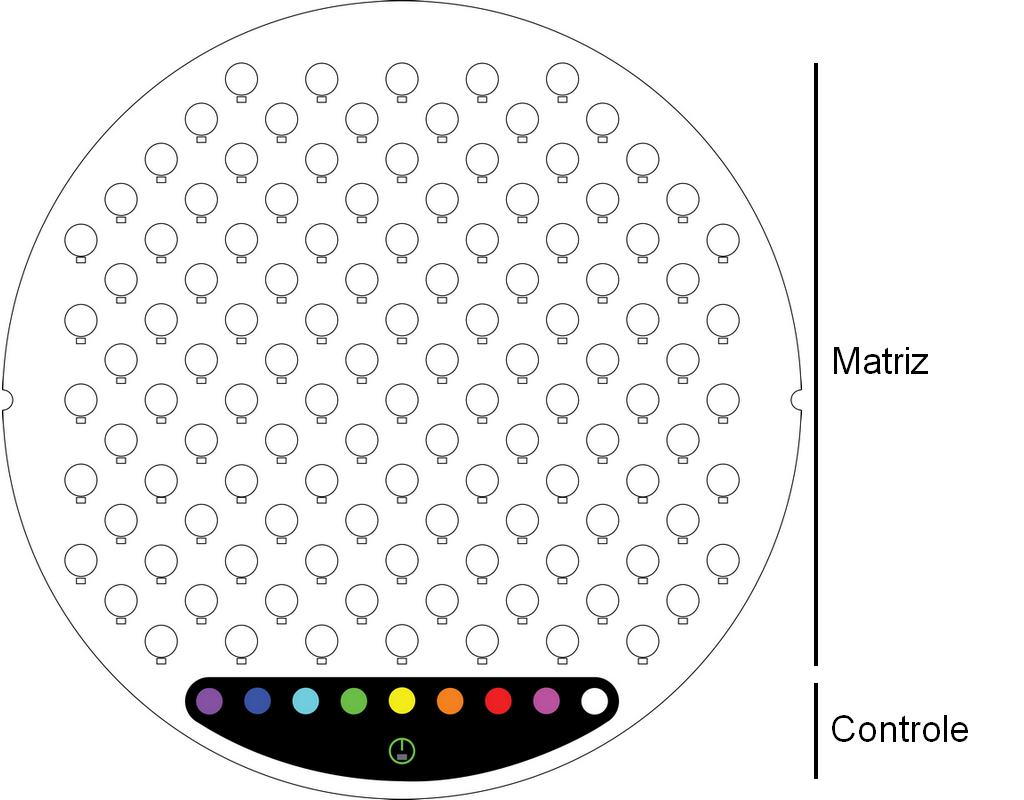
\includegraphics[width=0.7\textwidth]{./dados/figuras/mesa-cad}
    \fonte{(MITSUKO, 2016)}
    \label{fig:mesa-sup}
\end{figure}

\section{JUSTIFICATIVA}
\label{sec:justificativa}

  Sendo parte da exposição Luz, Ciência e Emoção, espera-se que o projeto fomente o envolvimento com a arte generativa e com as tecnologias envolvendo luz. Além de poder ser prestigiado durante a mostra, trata-se também de um projeto de código e \emph{hardware} abertos, que serão disponibilizados à comunidade para que possam ser estudados e adaptados às suas necessidades.

  Ademais, temas pouco explorados durante a graduação serão implementados, tais como técnica de contorno (\emph{debounce}, identificação de comandos reais sob contextos com ruído), padrão de \emph{design} em \emph{software} (FSM, máquina de estados finita) e geração de múltiplos canais de PWM.

\section{OBJETIVOS}
\label{sec:objetivos}

\subsection{OBJETIVO GERAL}
Finalizar o \emph{hardware} (seção Controle) e desenvolver o \emph{firmware} embarcado da Mesa de Bolinhas, apresentando um protótipo funcional do projeto.

\subsubsection{OBJETIVOS ESPECÍFICOS}
  \begin{itemize}
      \item Mapeamento da matriz de saída, onde cada \emph{LED} possa ser controlado individualmente;
      \item Mapeamento da matriz de entrada, onde cada sensor possa ser lido individualmente;
      \item \emph{Software} microcontrolado que gerencie a interface humano-máquina;
      \item Leiaute e montagem das Placas de Circuito Impresso;
      \item Integração da eletrônica com a mecânica do projeto.
  \end{itemize}
